% Bar charts
% Author: Stefan Kottwitz
% https://www.packtpub.com/hardware-and-creative/latex-cookbook
\documentclass[border=10pt]{standalone} 
%%%<
\usepackage{verbatim}
%%%>
\begin{comment}
:Title: Bar chart
:Tags: Charts;Cookbook
:Author: Stefan Kottwitz
:Slug: bar-chart

A bar chart can be used for comparing values.
Here we create a horizontal bar chart.

The pgfplots package provides an easy way.
In this example, I reduced axis data to
focus on the values. So I do not show
x-axis and y-axis, or axis ticks.
\end{comment}
\usepackage{pgfplots}
\begin{document}
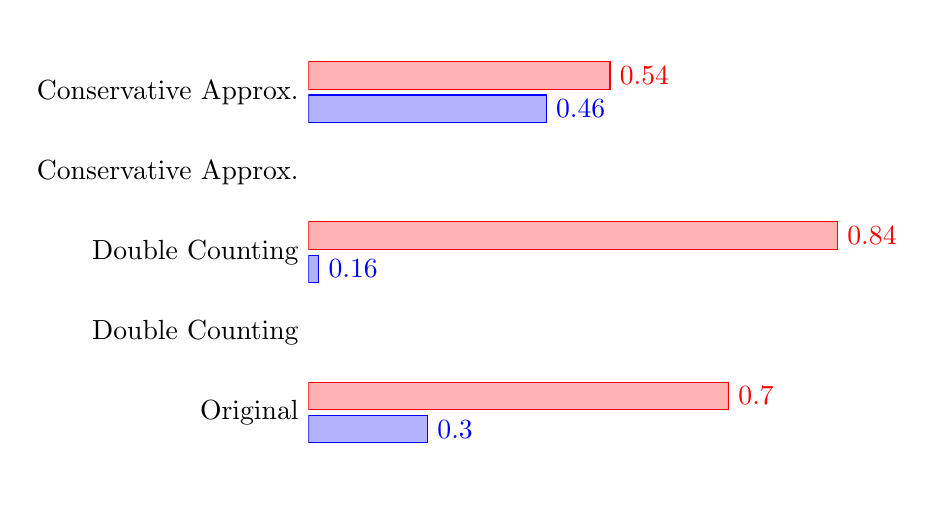
\begin{tikzpicture}
  \begin{axis}[
    xbar,
    y axis line style = { opacity = 0 },
    axis x line       = none,
    tickwidth         = 0pt,
    enlarge y limits  = 0.2,
    enlarge x limits  = 0.02,
    symbolic y coords = {Original, Double Counting, Conservative Approx.},
    nodes near coords,
  ]
  \addplot coordinates { (0.3,Original)   (0.1552,Double Counting) (0.4577,Conservative Approx.)   };
  \addplot coordinates { (0.7,Original)   (0.8448,Double Counting) (0.5423,Conservative Approx.)   };
  \end{axis}
\end{tikzpicture}
\end{document}